\begin{figure}[!htb]
  \centering
  %\begin{subfigure}[b]{0.15\textwidth}
    \begin{tikzpicture}[scale=1.0,auto,swap]

    % the two brain figures on top
    \node (upper_brain) at (0,1.5) { \includegraphics*[scale=\scaleBrainImg,trim=0 0 240 0]{images/dd15Sim2AD/stage_3.eps}};
    \node (lower_brain) at (0,-1.5) { \includegraphics*[scale=\scaleBrainImg,trim=240 0 0 0]{images/dd15Sim2AD/stage_3.eps}};
    \node[above=0cm of upper_brain] (stage) {Stage 3};
    % the balls
    
    \end{tikzpicture}
  %\end{subfigure}
  % next subfigure
  \hspace{-1.5em}
  ~
  %\begin{subfigure}[b]{0.15\textwidth}
    \begin{tikzpicture}[scale=1.0,auto,swap]

    % the two brain figures on top
    \node (upper_brain) at (0,1.5) { \includegraphics*[scale=\scaleBrainImg,trim=0 0 240 0]{images/dd15Sim2AD/stage_6.eps}};
    \node (lower_brain) at (0,-1.5) { \includegraphics*[scale=\scaleBrainImg,trim=240 0 0 0]{images/dd15Sim2AD/stage_6.eps}};
    \node[above=0cm of upper_brain] (stage) {Stage 6};
    % the balls
    
    \end{tikzpicture}
  %\end{subfigure}
  % next subfigure
  \hspace{-1.5em}
  ~
  %\begin{subfigure}[b]{0.15\textwidth}
    \begin{tikzpicture}[scale=1.0,auto,swap]

    % the two brain figures on top
    \node (upper_brain) at (0,1.5) { \includegraphics*[scale=\scaleBrainImg,trim=0 0 240 0]{images/dd15Sim2AD/stage_9.eps}};
    \node (lower_brain) at (0,-1.5) { \includegraphics*[scale=\scaleBrainImg,trim=240 0 0 0]{images/dd15Sim2AD/stage_9.eps}};
    \node[above=0cm of upper_brain] (stage) {Stage 9};
    % the balls
    
    \end{tikzpicture}
  %\end{subfigure}
  % next subfigure
  \hspace{-1.5em}
  ~
  %\begin{subfigure}[b]{0.15\textwidth}
    \begin{tikzpicture}[scale=1.0,auto,swap]

    % the two brain figures on top
    \node (upper_brain) at (0,1.5) { \includegraphics*[scale=\scaleBrainImg,trim=0 0 240 0]{images/dd15Sim2AD/stage_12.eps}};
    \node (lower_brain) at (0,-1.5) { \includegraphics*[scale=\scaleBrainImg,trim=240 0 0 0]{images/dd15Sim2AD/stage_12.eps}};
    \node[above=0cm of upper_brain] (stage) {Stage 12};
    % the balls
    
    \end{tikzpicture}
  %\end{subfigure}
  % next subfigure
  \hspace{-1.5em}
  ~
  %\begin{subfigure}[b]{0.15\textwidth}
    \begin{tikzpicture}[scale=1.0,auto,swap]

    % the two brain figures on top
    \node (upper_brain) at (0,1.5) { \includegraphics*[scale=\scaleBrainImg,trim=0 0 240 0]{images/dd15Sim2AD/stage_15.eps}};
    \node (lower_brain) at (0,-1.5) { \includegraphics*[scale=\scaleBrainImg,trim=240 0 0 0]{images/dd15Sim2AD/stage_15.eps}};
    \node[above=0cm of upper_brain] (stage) {Stage 15};
    % the balls
    
    \end{tikzpicture}
  %\end{subfigure}
  % next subfigure
  \hspace{-1.5em}
  ~
  \hspace{1em}
  % the red-to-yellow gradient on the right
  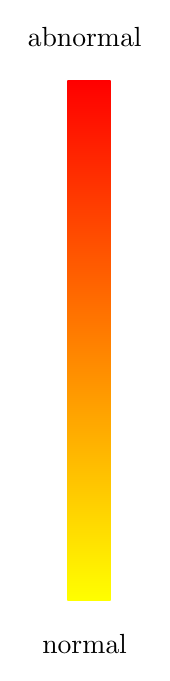
\begin{tikzpicture}[scale=1.1,auto,swap]
    \shade[top color=red,bottom color=yellow] (0,0) rectangle (0.5,6);
    \node[inner sep=0] (corr_text) at (0.2,6.5) {abnormal};
    \node[inner sep=0] (corr_text) at (0.2,-0.5) {normal};
  \end{tikzpicture}
  \caption[Atrophy progression snapshots for AD subjects using the data-driven EBM]{Brain atrophy snapshots for the AD subjects using the data-driven EBM at various stages in the disease progression: 3,6,9,12 and 15. The positional variance matrix used is the one from sampling method 2 from figure \ref{fig:dd_simultR}. The model suggests that in AD patients the cuneus/lingual gyrus, middle frontal gyrus, and the motor cortex become abnormal first, followed by areas in the posterior cortex. }
  \label{fig:snap_dd15_sim2_ad}
\end{figure}
